\documentclass[a4paper, 10pt, final, garamond]{book}
\usepackage{cours-preambule}
\graphicspath{{./figures/}}

\makeatletter
\renewcommand{\@chapapp}{Contr\^ole de connaissances}
\makeatother

\toggletrue{student}
% % \HideSolutionstrue
% \toggletrue{corrige}
\renewcommand{\mycol}{black}

\begin{document}
\setcounter{chapter}{16}

\chapter{Énergie et particules chargées\ifstudent{ (10')}}

\begin{enumerate}[label=\sqenumi]
	\nitem{2}%
	Comment trouver les points d'équilibre d'un système à partir de son énergie
	potentielle~? Quelle est la condition pour qu'un point d'équilibre soit
	stable~? Instable~?
	\smallbreak
	\psw{
		\[
			\text{Équilibre} \Lra
			\eval{\pdv{\Ec_p}{x}}_{x\ind{eq}} \stm{=} 0
			\qet \text{stable si} \eval{\pdv[2]{\Ec_p}{x}}_{x\ind{eq}} \stm{>} 0
			\quad ; \quad
			\text{instable si} \eval{\pdv[2]{\Ec_p}{x}}_{x\ind{eq}} < 0
		\]
	}
	\nitem{6}%
	Démontrer le théorème de l'énergie mécanique. Utiliser le TEM pour retrouver
	la vitesse d'une skieuse en bas d'une piste de dénivelé $h$ avec une vitesse
	initiale nulle.
	\smallbreak
	\begin{isd}
		\tcbsubtitle{\fatbox{\textbf{TEM}}}
		\vspace{-15pt}
		\psw{
			\begin{DispWithArrows*}[fleqn, mathindent=-20pt]
				\Delta_{\ABr}{\Ec_c}
				&\stm{=}
				\sum_{n} W_{\ABr}(\Ff_{n})
				\\\Lra
				\D_{\ABr}\Ec_c
				&=
				\sum_j \underbracket[1pt]{W_\ABr(\Ff_{{\rm cons},j})}_{=-\D\Ec_{p,j} \pt{1}}
				+ \sum_i W_\ABr(\Ff_{{\rm NC}, i})
				\\\Lra
				\D_{\ABr}\Ec_c + \D_{\ABr}\Ec_{p,\tot}
				&=
				\boxed{
					\D_{\ABr}\Ec_m\Rg \stm[-1]{=}
					\sum_i W_{\ABr}(\Ff_{{\rm NC},i})
				}
			\end{DispWithArrows*}
		}
		\tcblower
		\psw{
			\begin{gather*}
				\beforetext{En haut}
				\Ec_m(\Ar) = \frac{1}{2}mv_{\Ar}{}^2 + mgz_{\Ar} = 0 + mgh
				\\
				\beforetext{En bas}
				\Ec_m(\Br) = \frac{1}{2}mv_{\Br}{}^2 + mgz_{\Br} \stm{=} \frac{1}{2}mv^2 + 0
				\\
				\beforetext{Or}
				W_{\ABr}(\Nf) \stm[-1]{=} 0 = \Delta_{\ABr}\Ec_{m}
				\\\Ra
				\frac{1}{2}mv^2 = mgh \quad\Ra\quad \boxed{v \stm[-1]{=} \sqrt{2gh}}
			\end{gather*}
		}
		\vspace{-15pt}
	\end{isd}
	\nitem{5}%
	Quelles sont les régions accessibles par un système d'énergie totale $\Ec_m$
	dans un diagramme d'énergie potentielle~? Comment repère-t-on que le système a
	une vitesse nulle~? maximale~? Représenter deux diagrammes d'énergie
	potentielle présentant un état lié et un état de diffusion.
	\smallbreak
	\begin{isd}[lefthand ratio=.3]
		\begin{itemize}
			\litem{10pt}{\pt{1}}%
			\psw{Seules les régions où $\Ec_p \leq \Ec_m$ sont accessibles~;}
			\litem{10pt}{\pt{1}}%
			\psw{
				Lorsque $\Ec_p = \Ec_m$, $\Ec_c = 0$ donc la vitesse est nulle~;
			}
			\litem{10pt}{\pt{1}}%
			\psw{
				Lorsque $\Ec_p$ est minimale, $\Ec_c$ est maximale.
			}
		\end{itemize}
		\tcblower
		\begin{isd}[sidebyside align=top]
			\begin{center}
				\sswitch{
					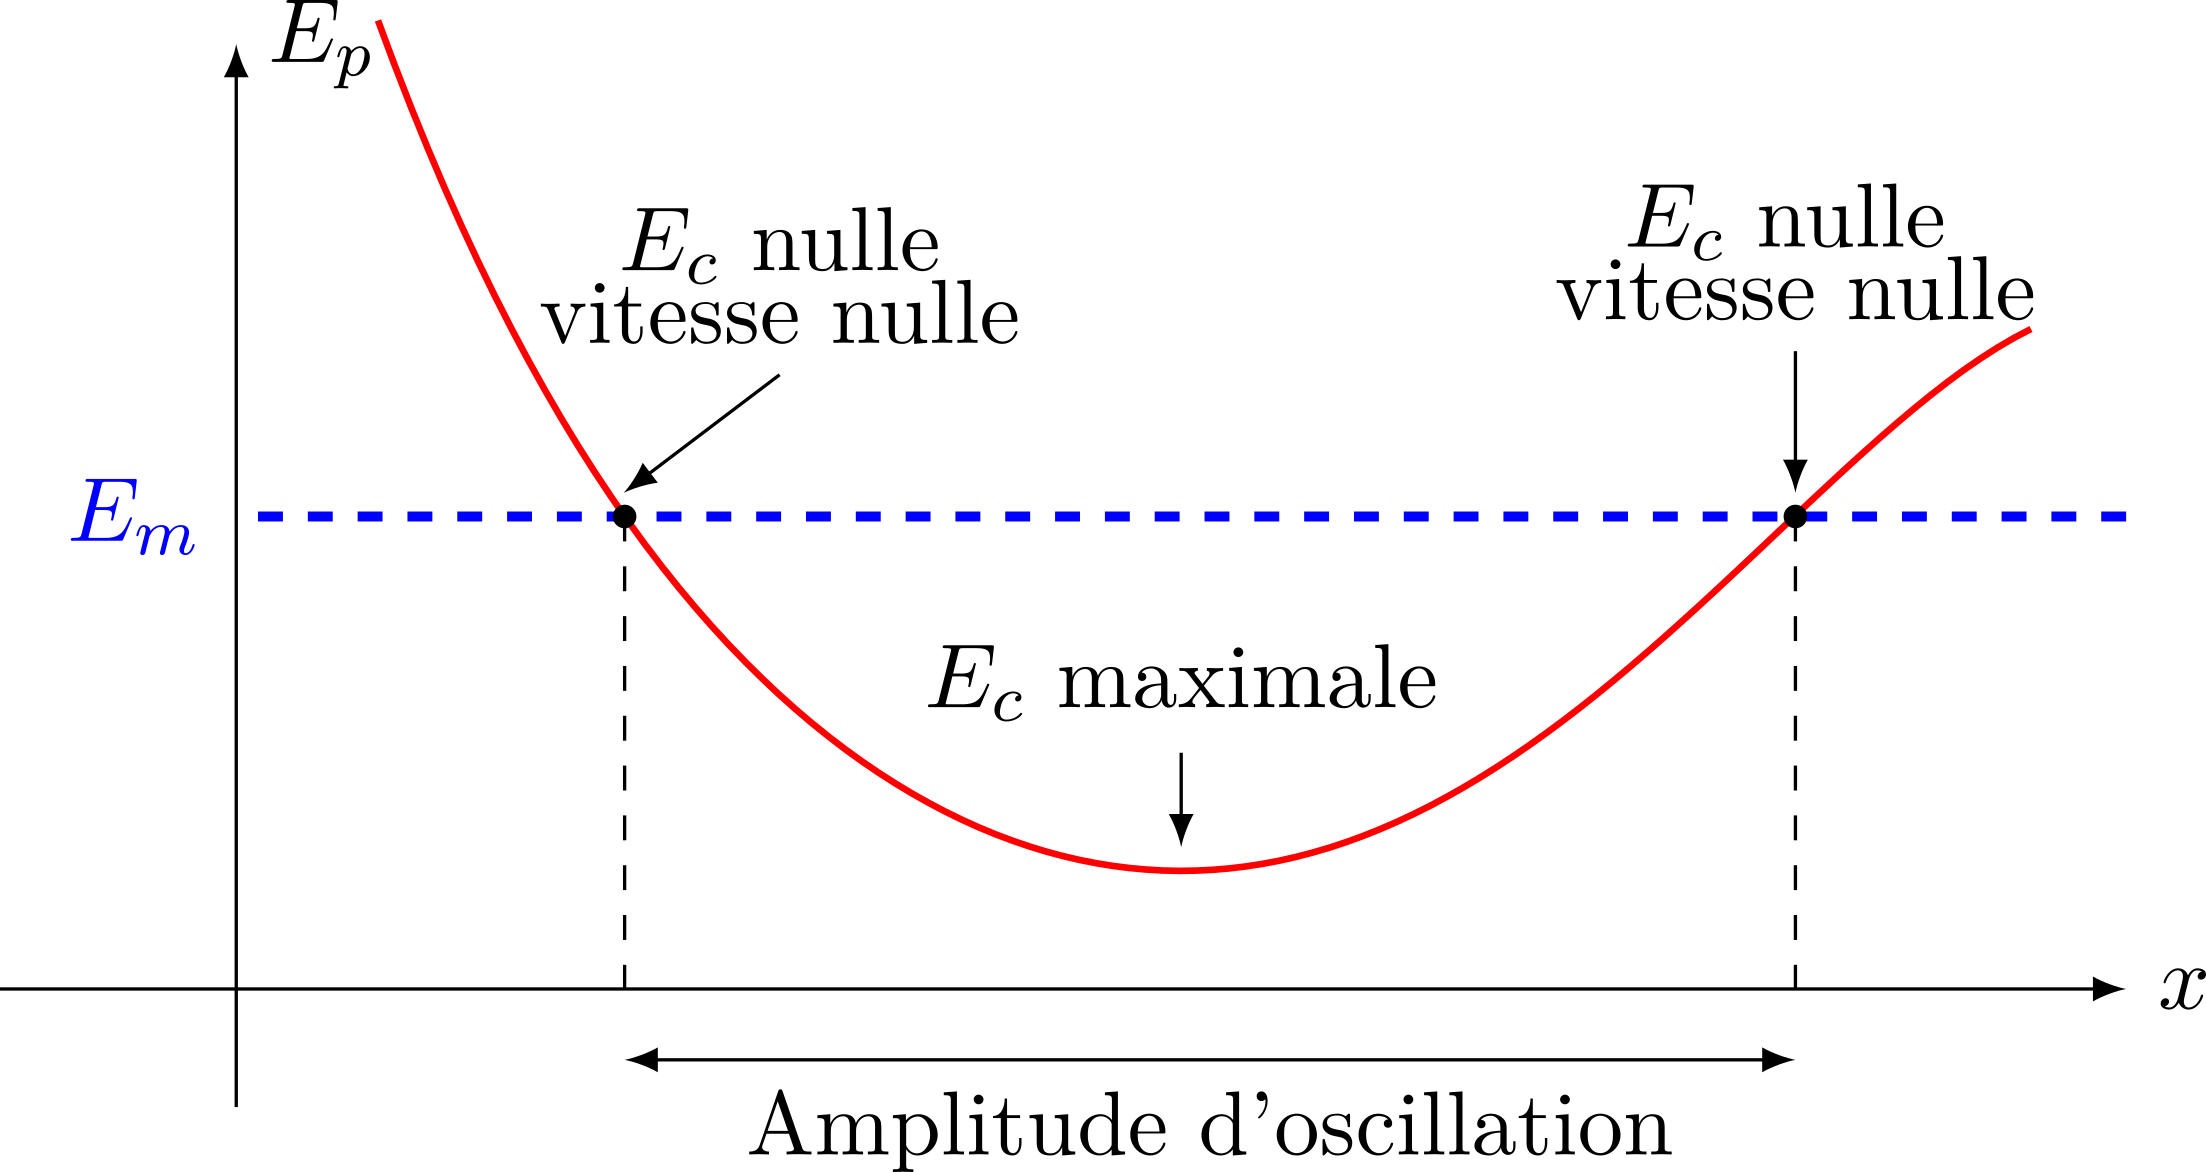
\includegraphics[width=\linewidth, draft=true]{stab_lie}
				}{
					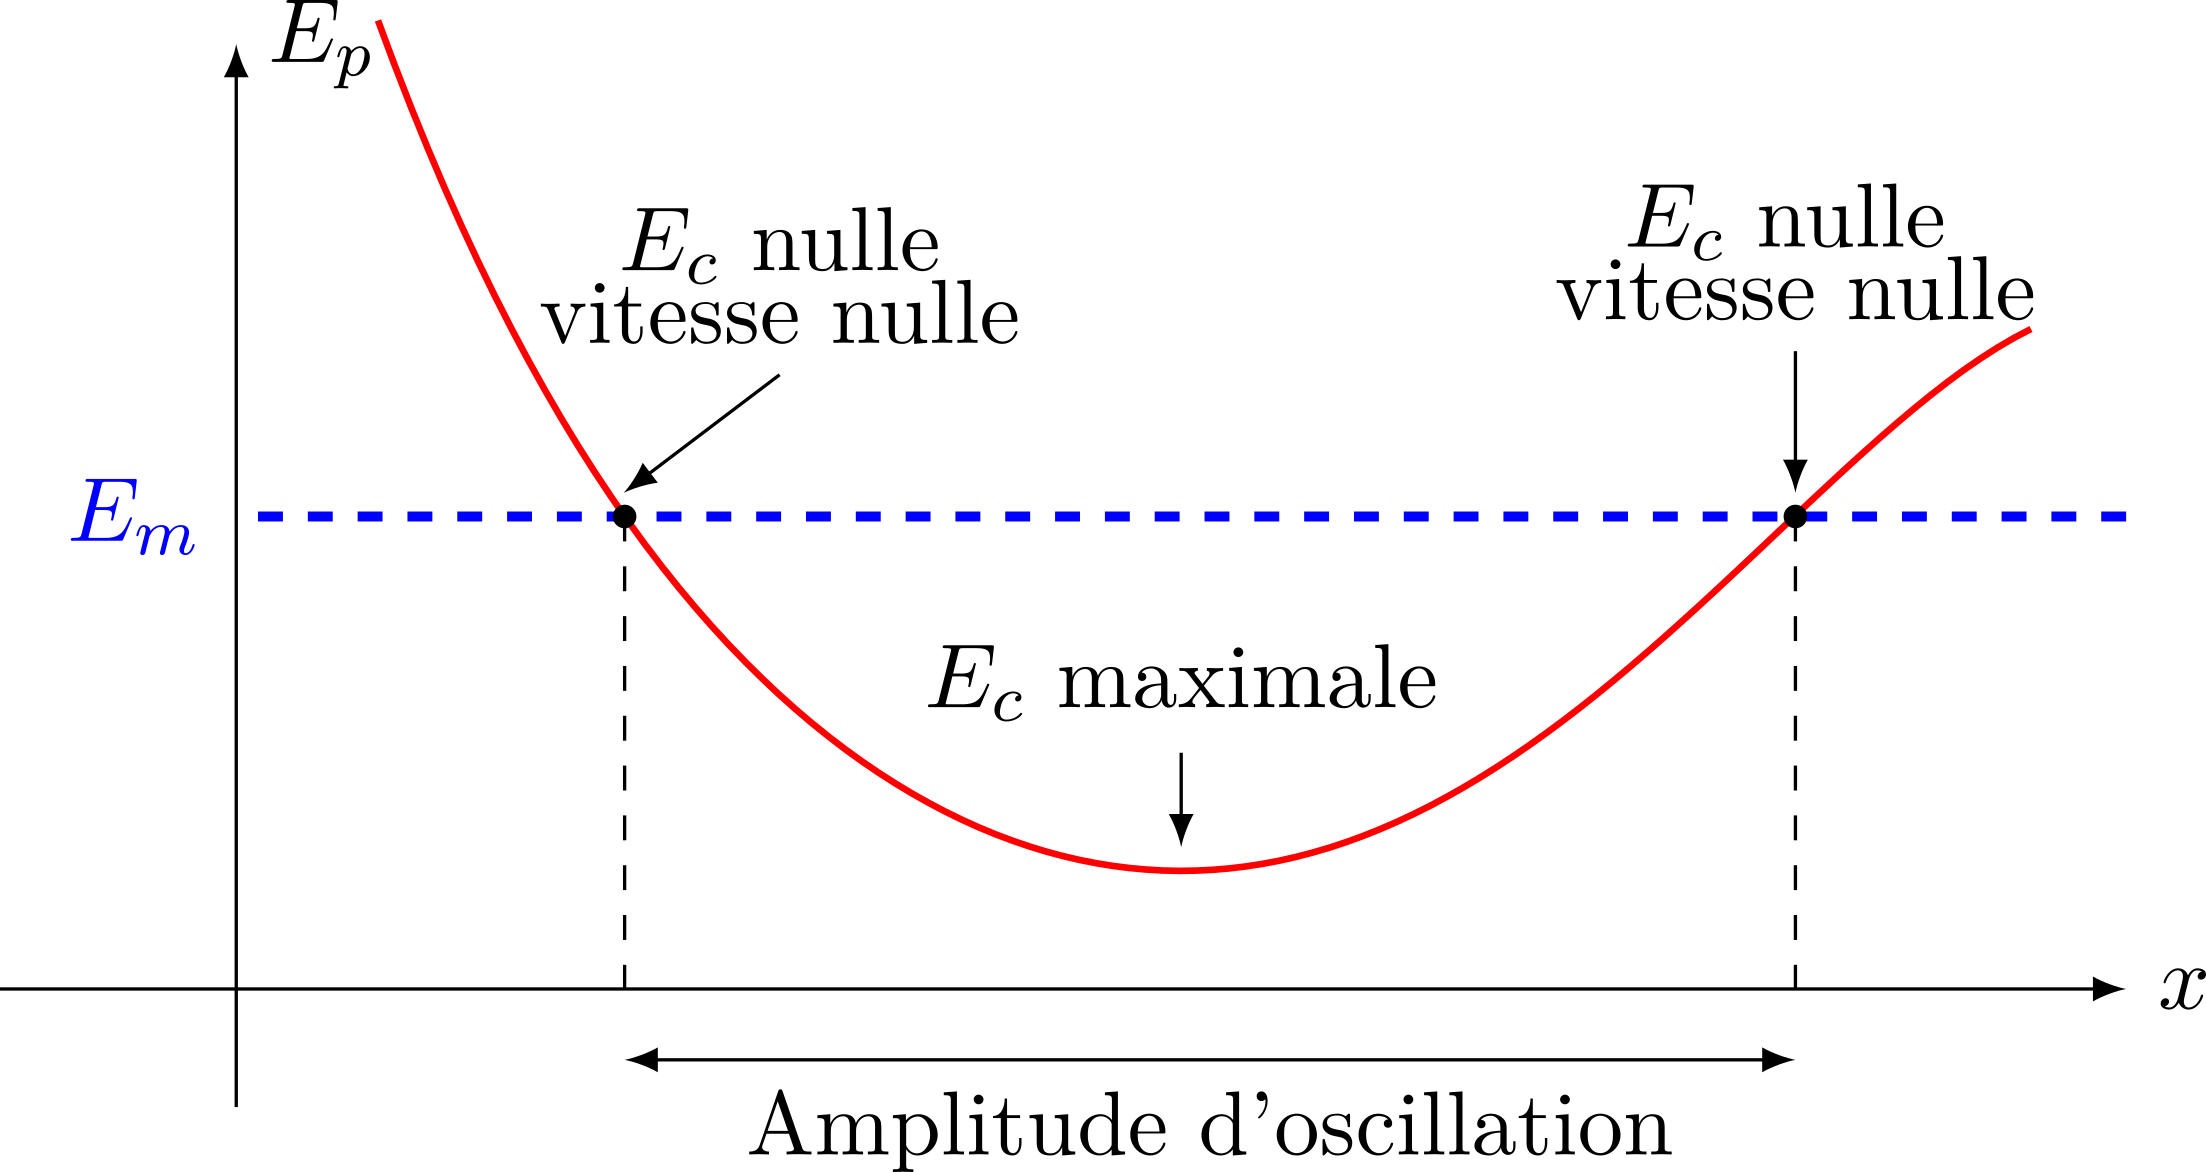
\includegraphics[width=\linewidth]{stab_lie}
				}
				\captionof{figure}{État lié \protect\pt{1}}
			\end{center}
			\tcblower
			\begin{center}
				\sswitch{
					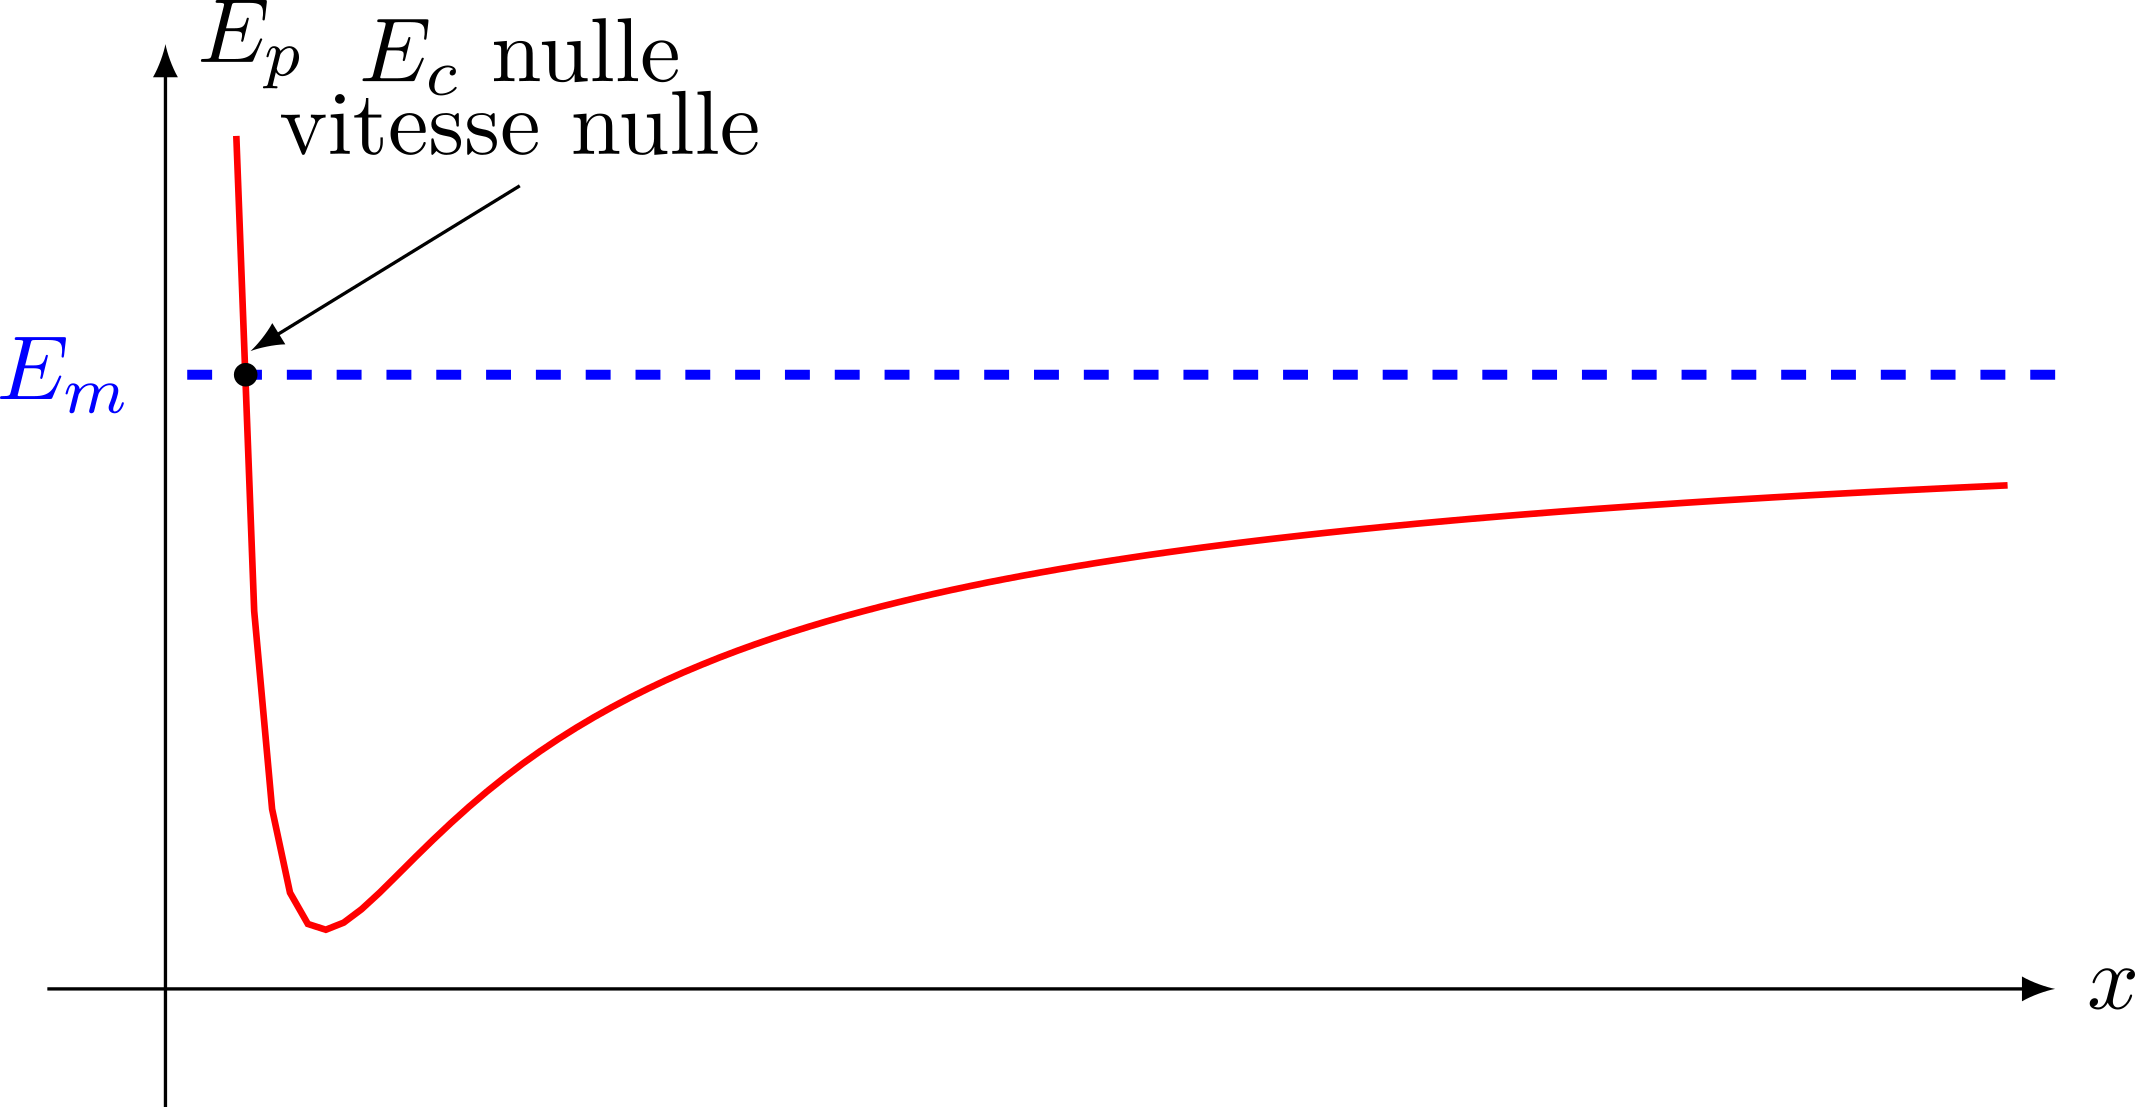
\includegraphics[width=\linewidth, draft=true]{stab_diff}
				}{
					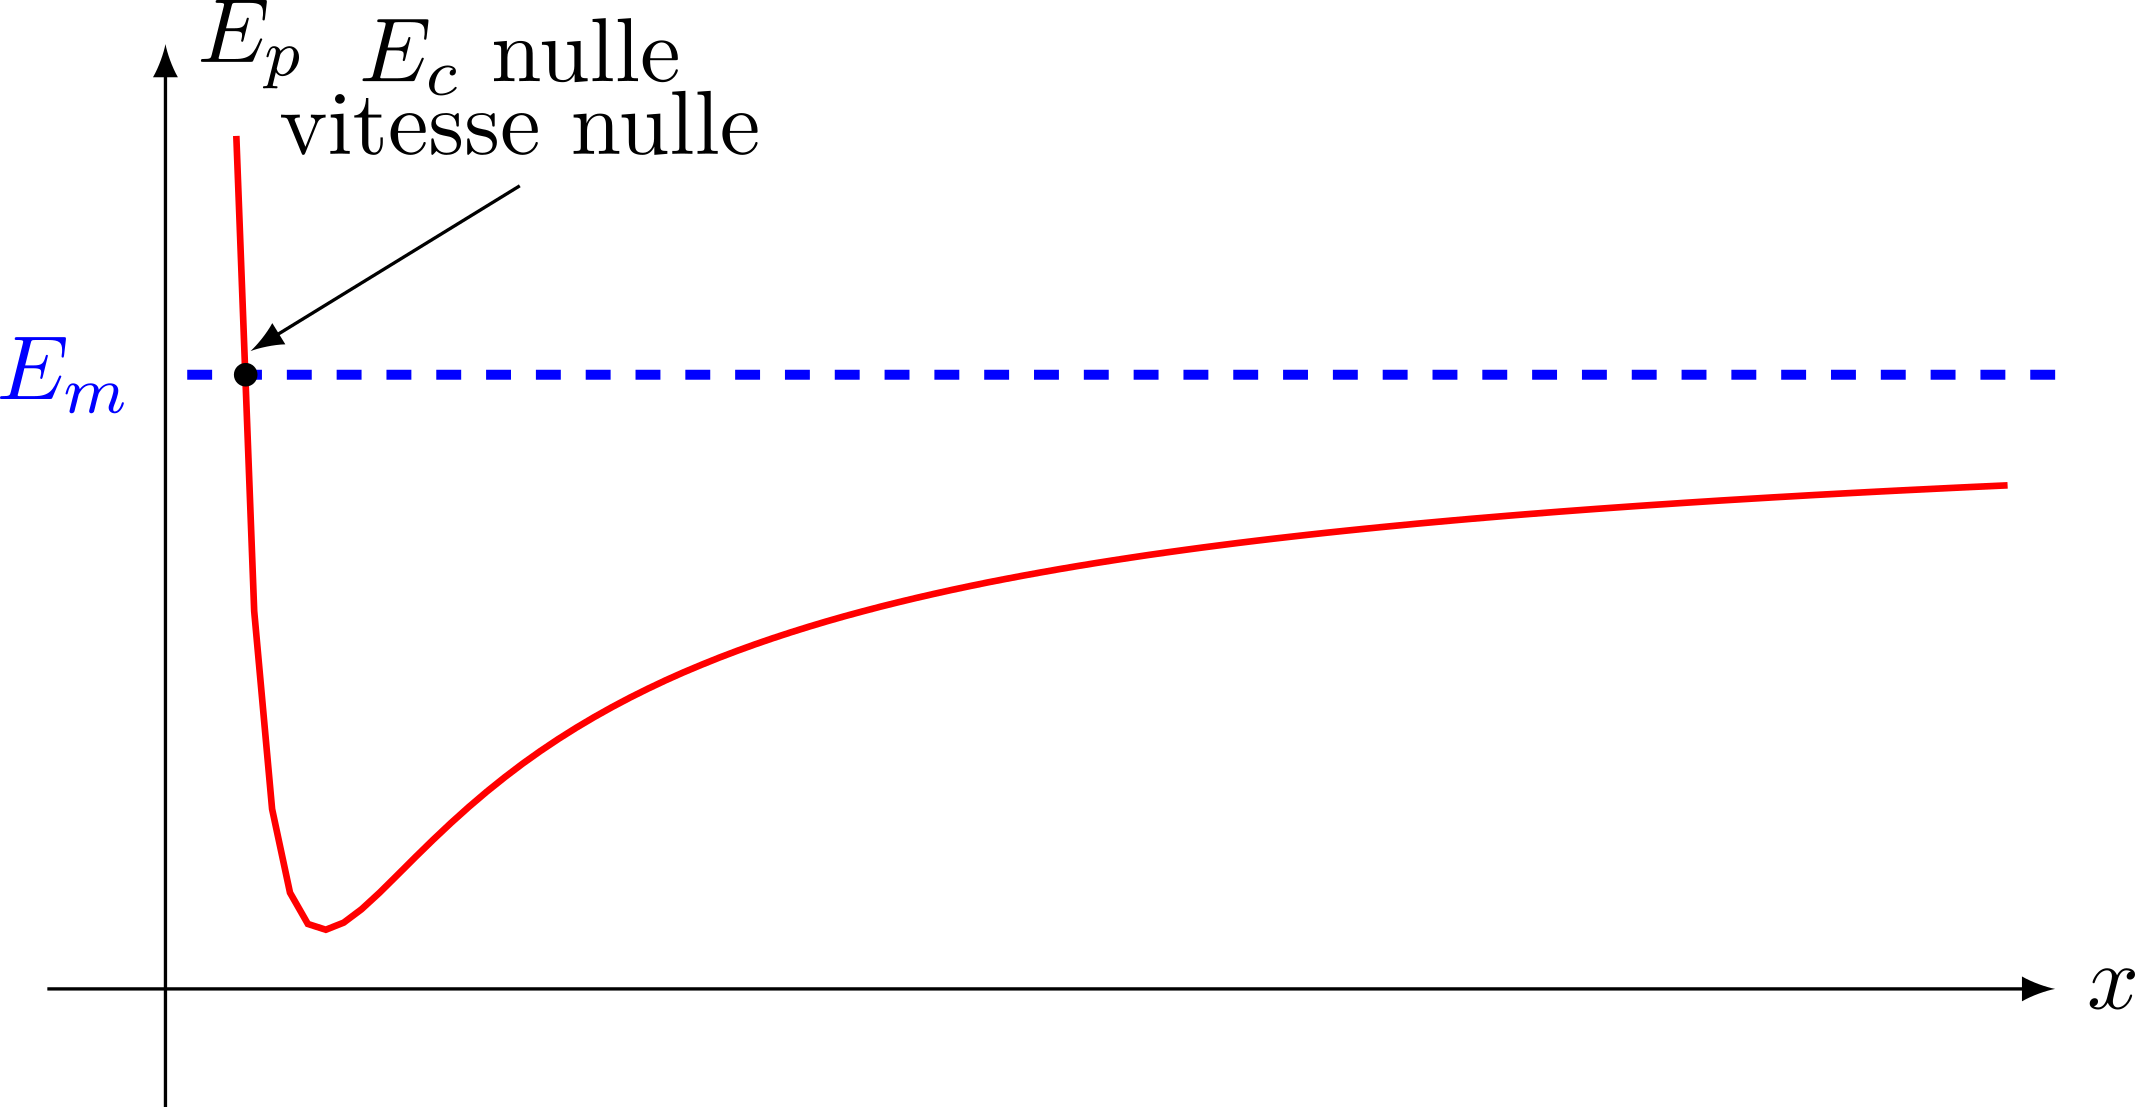
\includegraphics[width=\linewidth]{stab_diff}
				}
				\captionof{figure}{État de diffusion\protect\pt{1}}
			\end{center}
		\end{isd}
	\end{isd}
	\nitem{3}%
	Donner l'expression de la force de \textsc{Lorentz}. Montrer que la force
	magnétique ne modifie pas la vitesse d'une particule chargée en calculant la
	puissance de la force de \textsc{Lorentz}.
	\smallbreak
	\vspace{-15pt}
	\psw{
		\[
			\Ff \stm{=} q \left( \Ef + \vf \wedge \Bf \right)
			\Ra
			\Pc(\Ff) = q \left( \Ef + \vf \wedge \Bf \right)\cdot \vf
			= q\Ef\cdot\vf +
			q\underbracket[1pt]{\underbracket[1pt]{\vf\wedge\Bf}_{\perp\vf}\cdot\vf}_{=0}
			\Lra
			\boxed{\Pc(\Ff) \stm[-1]{=} q\Ef\cdot\vf} \stm{=} \dv{\Ec_c}{t}
		\]
	}
	\vspace{-15pt}
	\nitem{4}%
	On suppose une particule chargée positivement, arrivant en $z = 0$ à la vitesse
	$\vfo = v_0\uz$ dans un champ électrique $\Ef = E \uz$, créé par une tension
	$U$ entre les potentiels $V(0)$ et $V(d)$. Déterminer la vitesse de la
	particule en sortie.
	\smallbreak
	\vspace{-15pt}
	\psw{
		\begin{gather*}
			\Ec_m(0) = \frac{1}{2}mv_0{}^2 + qV(0)
			\qquad \text{et} \pt{1} \qquad
			\Ec_m(d) = \frac{1}{2}mv_f{}^2 + qV(d)
			\\
			\beforetext{Système conservatif \pt{1} $\Ra$}
			\frac{1}{2}mv_0{}^2 + qV(0) \stm[-1]{=} \frac{1}{2}mv_f{}^2 + qV(d)
			\\\Lra
			v_f{}^2 = v_0{}^2 + \frac{2q}{m}\left(V(0) - V(d)\right)
			\\\Lra
			\boxed{v_f \stm[-1]{=} \sqrt{v_0{}^2 + \frac{2qU}{m}}}
		\end{gather*}
	}
	\ifstudent{
		\begin{tikzpicture}[remember picture, overlay]
			\node[anchor=north west, align=left]
			at ([shift={(1.4cm,0)}]current page.north west)
			{\\[5pt]\Large\bfseries Nom~:\\[10pt]\Large\bfseries Prénom~:};
			\node[anchor=north east, align=right]
			at ([shift={(-1.5cm,-17pt)}]current page.north east)
			{\Large\bfseries Note~:\hspace{1cm}/20};
		\end{tikzpicture}
	}
\end{enumerate}
\end{document}
